\subsection{Oracle VM VirtualBox}\label{vbox}

\begin{wrapfigure}{r}{0.2\textwidth} %this figure will be at the right
    \centering
    
\includegraphics[width=0.2\textwidth]{../images/vbox.png}
\end{wrapfigure}

VirtualBox é um software de virtualização que pode ser instalado em diversos sistemas hospedeiros e tem como objetivo gerenciar máquinas virtuais.

Para este manual, a versão do VirtualBox que está sendo executado é a 6.0.8 em um hospedeiro Windows, e foi o software escolhido para executar a imagem do ambiente Linux Alpine onde é executado o sistema de buscas.

Após a instalação do software\footnotetext{\url{https://www.virtualbox.org/wiki/Downloads}} e dada uma imagem \lstinline{.ova}, para replicar o ambiente no VirtualBox, é necessário:
\begin{enumerate}
    \item Escolher a opção do menu \textit{Import Appliance}.
     \begin{figure}[H]
        \centering
        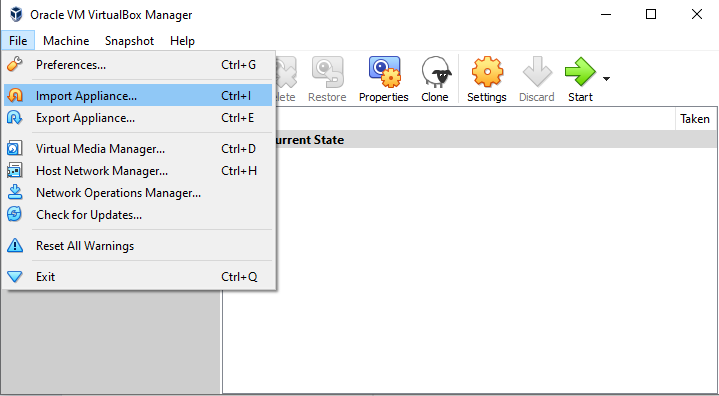
\includegraphics[width=0.5\textwidth]{images/vbox1.png}
    \end{figure}
    \item Escrever o caminho da imagem do Alpine \lstinline{.ova}.
    \item Selecionar a opção \textit{Import} para uma importação básica do sistema. Após esse processo, espere o processo de importação terminar.
\end{enumerate}

Se a imagem foi instalada corretamente, clique em \textit{Start} no menu principal do VirtualBox e aguardea tela de boas vindas ilustrada na Figura \ref{fig1}.
\begin{figure}[H]
    \centering
    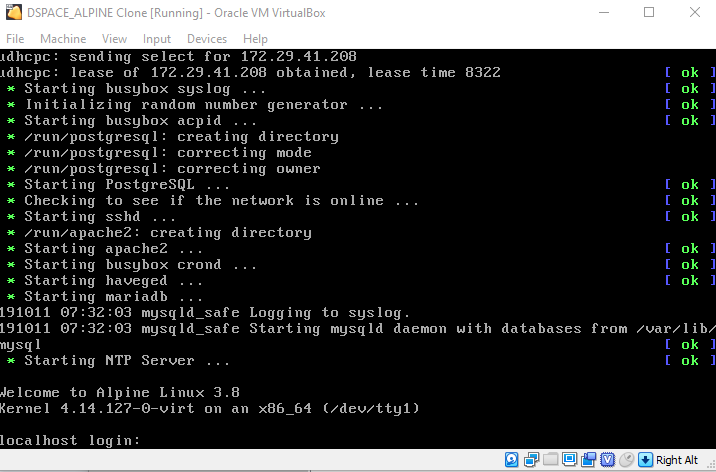
\includegraphics[width=0.5\textwidth]{images/vbox2.png}
    \caption{Tela de Boas-Vindas.}
    \label{fig1}
\end{figure}

Considerando que nenhuma outra configuração no VirtualBox foi feita além das explicadas neste manual, utilize a tecla \textit{AltGr} para alternar o foco entre o sistema hospedeiro e o sistema cliente. 

\subsection{Alpine Linux}\label{alpine}

 \begin{wrapfigure}{r}{0.2\textwidth} %this figure will be at the right
     \centering
     
\includegraphics[width=0.2\textwidth]{../images/alpine.png}
     \label{fig2}
 \end{wrapfigure}

Alpine é uma distribuição Linux para uso não-comerciais, com o foco em eficiência e simplicidade, possuindo apenas recursos básicos e necessários para o ambiente Linux.

A versão utilizada neste sistema é a 3.8, sendo uma imagem de extensão \lstinline{.ova}, que pode ser simulada no programa VirtualBox, explicado na Seção \ref{vbox}. Assim que o sistema é inicializado, é exigido um login e uma senha para utilizar o ambiente. 

\begin{lstlisting}[language=bash, label=lst1, caption=Login e senha de acesso]
    localhost login: dspace
    Password: dspace
\end{lstlisting}

Os principais programas que devem inicializar juntamente com o Alpine são:

\begin{itemize}
    \item Tomcat, seção \ref{tomcat}.
    \item Apache, seção \ref{apache}.
\end{itemize}

Para utilizar os recursos do Alpine na máquina hospedeira, recomenda-se o programa Putty, explicado na Seção \ref{conexao}.

Para transferir arquivos entre a máquina hospedeira e o Alpine, recomenda-se o programa Filezilla, explicado na Seção \ref{transfer}.

\subsubsection{Gerenciamento de pacotes}

O Alpine utiliza o sistema de gerenciamento de pacotes \lstinline{apk}, que pode ser lido em mais detalhes em \url{https://wiki.alpinelinux.org/wiki/Alpine_Linux_package_management}.

A lista dos repositórios de pacotes disponíveis do Alpine podem ser editados utilizando o editor \textit{vim} com o comando:

\begin{lstlisting}[language=bash]
    vim /etc/apk/repositories
\end{lstlisting}

Atualmente, a versão dos repositórios escolhidos para baixar os pacotes é a \textbf{3.3}, disponíveis em \url{http://mirror.math.princeton.edu/pub/alpinelinux/}, que até o momento possuía o pacote \textbf{php-apache} e o pacote \textbf{php-mysql}, os quais foram essenciais para a instalação do sistema Tematres, explicado na Seção \ref{tematres}.

\subsubsection{Conexão entre máquina hospedeira e a imagem}\label{conexao}

\begin{wrapfigure}{r}{0.2\textwidth} %this figure will be at the right
    \centering
    
\includegraphics[width=0.2\textwidth]{../images/putty1.png}
\end{wrapfigure}

Putty é um software de emulação de terminal que suporta conexões SSH e telnet. Desta forma, fica mais simples manipular o cliente, no caso deste manual, o Alpine, sem necessariamente utilizar a máquina virtual, a qual está rodando no VirtualBox.

Para utilizar o Putty juntamente com a imagem do Alpine disponibilizada, utilize o comando \lstinline{ifconfig} para descobrir o endereço \textit{inet} e fazer a conexão entre o Putty e o terminal do alpine.

 \begin{figure}[H]
 
     \begin{subfigure}{0.6\textwidth}
     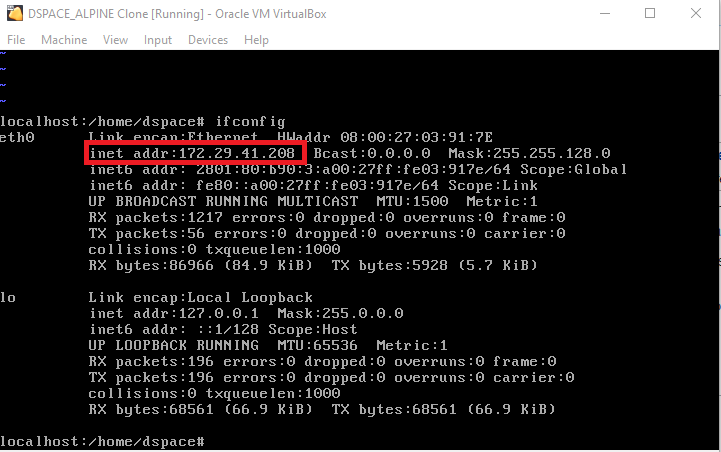
\includegraphics[width=0.9\linewidth]{../images/putty2.png} 
     \caption{ifconfig.}
     \end{subfigure}
     \begin{subfigure}{0.4\textwidth}
     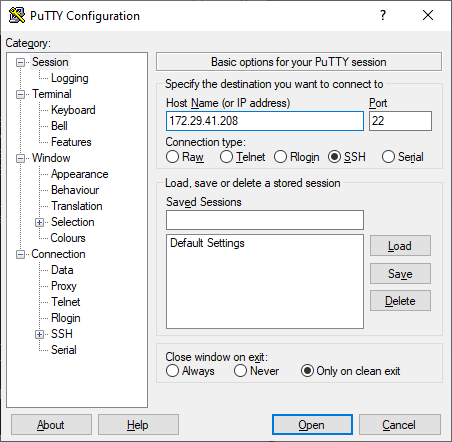
\includegraphics[width=0.9\linewidth]{../images/putty3.png}
     \caption{Configuração do putty.}
     \end{subfigure}
 
 \caption{Utilizando Putty.}
 \end{figure}

 No Putty, edite o campo \textit{Host Name (or IP adress)} com o endereço \textit{inet} fornecido, confira se a porta selecionada é a \textit{22} e se o tipo de conexão é \textit{SSH}. Após isso, clique em \textbf{Open}.

 Irá aparecer um aviso sobre conexão não-segura, o qual pode ser ignorado. O login e a senha serão os mesmos informados na Listagem \ref{lst1}.

 \begin{figure}[H]
    \centering
    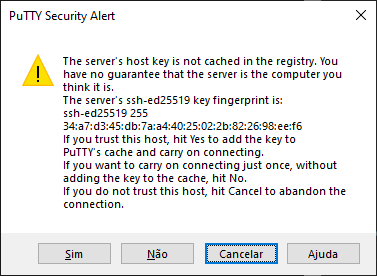
\includegraphics[width=0.5\textwidth]{images/putty4.png}
    \caption{Aviso de conexão não-segura. Clique em \textit{sim} para ignorar.}
    \label{fig1}
\end{figure}

Após isso, você poderá utilizar o terminal do Alpine na máquina hospedeira.

\subsubsection{Transferência de arquivos}\label{transfer}

\begin{wrapfigure}{r}{0.2\textwidth} %this figure will be at the right
    \centering
    
\includegraphics[width=0.2\textwidth]{../images/filezilla.jpg}
\end{wrapfigure}

Filezilla é um software para realizar transferências de arquivos utilizando o protocolo FTP \footnote{\url{https://filezilla-project.org/}}. Necessariamente, para transferir um arquivo de um servidor para o cliente, o diretório do cliente deve estar com permissão de leitura e escrita.

Para conectar o Filezilla com o Alpine, similar ao Putty, na Seção \ref{conexao}, edite os campos conforme a Listagem \ref{lst2}. Para o endereço do campo \textit{host}, utilize o comando \textit{ifconfig} para descobrir o endereço \textit{inet} .

\begin{lstlisting}[language=bash, label=lst2, caption=Campos do Filezilla para serem alterados]
    Host: <ENDERECO INET>
    Nome de usuario: dspace
    Senha: dspace
    Porta: 22
\end{lstlisting}

\begin{figure}[H]
    \centering
    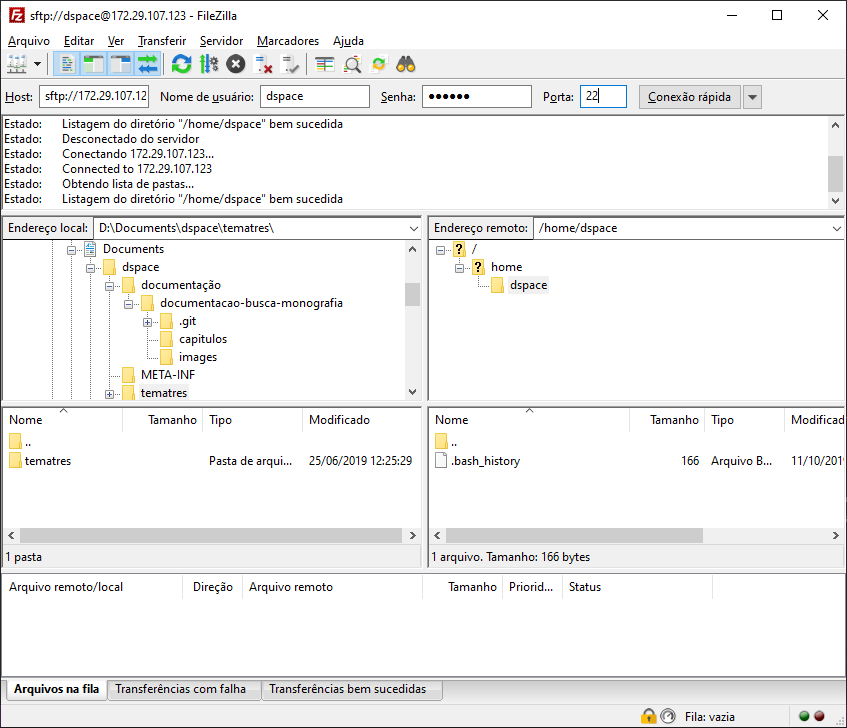
\includegraphics[width=0.5\textwidth]{images/filezilla1.png}
    \caption{Exemplo de conexão.}
    \label{fig1}
\end{figure}

Se conectado corretamente, o filezilla deve exibir o diretório \textit{dspace}. Na versão do Alpine que foi configurado no dia 10 de outubro, no diretório \textit{home}, existe um diretório chamado \textit{filezilla}, já configurado para permitir leitura, escrita e execução dos arquivos que serão transferidos para esta pasta. \todo{Inseguro. Configurar outro modo para usar filezilla}.

\begin{figure}[H]
    \centering
    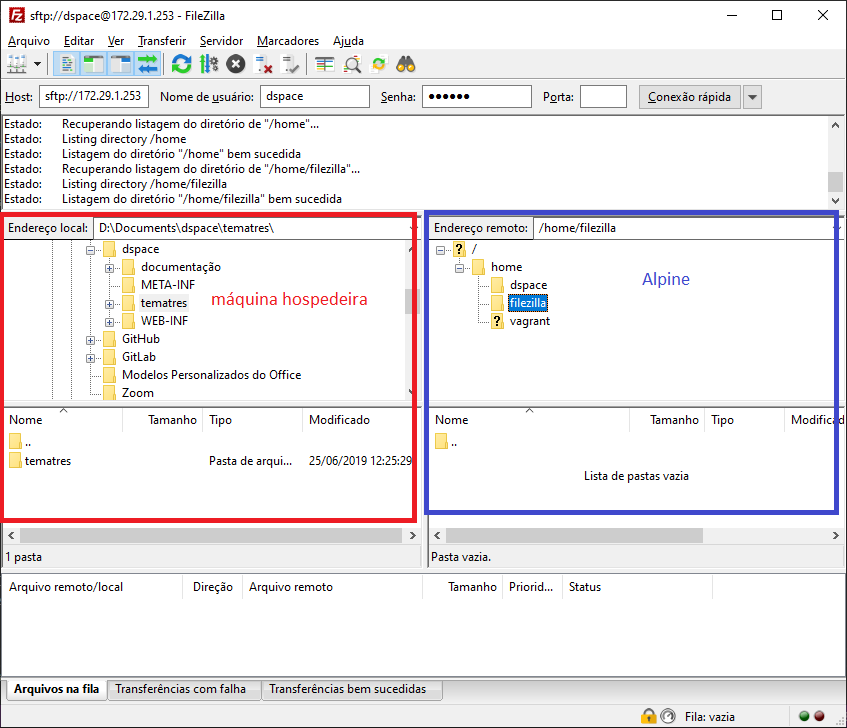
\includegraphics[width=0.5\textwidth]{images/filezilla2.png}
    \caption{Em vermelho, arquivos e diretório da máquina hospedeira. Em azul, arquivos e diretórios da máquina virtual.}
    \label{fig1}
\end{figure}

Para transferir arquivos entre a máquina hospedeira e o Alpine, selecione o arquivo que deseja transferir e arraste para a pasta \textit{filezilla}. Até o momento atual, o único diretório que aceita este tipo de transferência é o diretório \textit{filezilla}. Caso exista a necessidade de mover estes arquivos para outros diretórios no Linux, utilize o Putty, explicado na Seção \ref{conexao}, para mover estes arquivos por linha de comando.

\subsection{Tomcat}\label{tomcat}
\begin{wrapfigure}{r}{0.2\textwidth} %this figure will be at the right
    \centering
    
\includegraphics[width=0.2\textwidth]{../images/tomcat.png}
\end{wrapfigure}

Tomcat é um servidor web que cria um ambiente para executar páginas \textit{JSP} e dentre outras especificações do Java EE (incluindo os \textit{webapps}).

O Tomcat é utilizado para configurar o ambiente do DSpace, comentado em mais detalhes na Seção \ref{dspace}.

Para a versão \textit{20191010} da imagem do Alpine, o Tomcat conecta na porta 8081 do \textit{localhost}. Por padrão, a porta do Tomcat é a \textit{8080}, mas este valor foi alterado por motivos de testes para uma máquina rodar tanto o Tomcat quanto o Apache. Para configurar o servidor do Tomcat (para alterar a porta, por exemplo), utilize o comando da Listagem \ref{lst:server.xml}.

\begin{lstlisting}[language=bash, label=lst:server.xml, caption=Abrindo server.xml do Tomcat.]
    vim /usr/local/tomcat/conf/server.xml
\end{lstlisting}

Antes de inicializar os serviços do Tomcat, verifique se ele já está inicializado com o comando da Listagem \ref{lst:grep.tomcat}. Após usar este comando, o terminal deve imprimir uma mensagem parecida com a Listagem \ref{lst:grep.tomcat.resposta}.

\begin{lstlisting}[language=bash, label=lst:grep.tomcat, caption=Verificando se o TomCat está inicializado.]
    ps -ef | grep tomcat
\end{lstlisting}

\begin{lstlisting}[language=bash, breaklines=true, label=lst:grep.tomcat.resposta, caption=Parte de uma resposta de um Tomcat que já está rodando]
    2646 root      3:15 /usr/lib/jvm/java-1.8-openjdk/bin/java -Djava.util.logging.config.file=/usr/local/apache-tomcat-8.5.40/conf/logging.properties -Djava.util.logging.manager=org.apache.juli....
\end{lstlisting}

Caso o Tomcat não esteja inicializado, utilize o comando da Listagem \ref{lst:tomcat.start} para inicializar o Tomcat. Caso seja necessário encerrar o Tomcat, utilize o comando da Listagem \ref{lst:tomcat.shutdown}.

\begin{lstlisting}[language=bash, label=lst:tomcat.start, caption=Inicializando Tomcat.]
    /etc/init.d/tomcat start
\end{lstlisting}

\begin{lstlisting}[language=bash, label=lst:tomcat.shutdown, caption=Encerrando Tomcat.]
    /etc/init.d/tomcat stop
\end{lstlisting}

\subsection{PostgreeSQL}\label{postgree}
\begin{wrapfigure}{r}{0.2\textwidth} %this figure will be at the right
    \centering
    
\includegraphics[width=0.2\textwidth]{../images/postgree.png}
\end{wrapfigure}
PostgreeSQL é um gerenciador de banco de dados que lida com dados relacionais. Este foi escolhido como SGDB para lidar com dados do DSpace.

Atualmente, com a versão \textit{20191010} da imagem do Alpine, o Postgree inicializa juntamente com a inicialização da máquina Linux, não sendo necessário comandos para inicializar ou parar.

\todo{usuário para acessar banco}

\subsection{Apache}\label{apache}
\begin{wrapfigure}{r}{0.2\textwidth} %this figure will be at the right
    \centering
    
\includegraphics[width=0.2\textwidth]{../images/apache.jpg}
\end{wrapfigure}
Apache é um servidor web que possui diversas módulos para criar um ambiente para executar páginas de diferentes linguagens, como Perl e PHP.
O Apache é utilizando para configurar o ambiente do Tematres, comentado em mais detalhes na Seção \ref{tematres}. 

O Apache foi instalado utilizando os comandos da Listagem \ref{lst:apache.instalacao}. Ao instalar o Apache, também instalou-se o PHP e o MySQL, comentando em mais detalhes na Seção \ref{php} e na Seção \ref{mysql}.

\begin{lstlisting}[language=bash, label=lst:apache.instalacao, caption=Instalando Apache.]
    apk add php-mysqli
    apk add php-ctype
\end{lstlisting}

Por padrão, a porta do Apache é a \textit{80}. Esta porta foi mantida na imagem \textit{20191010}.

\subsubsection{PHP}\label{php}
\begin{wrapfigure}{r}{0.2\textwidth} %this figure will be at the right
    \centering
    
\includegraphics[width=0.2\textwidth]{../images/php.png}
\end{wrapfigure}
PHP é uma linguagem de programação principalmente utilizada para o desenvolvimento web, utilizada em diversas aplicações. Dentre as aplicações, o Tematres.

Atualmente, duas versões do PHP foram instaladas de maneira equivocada na imagem do Alpine, mas apenas a versão \textbf{5.6.40} é interpretada pelo servidor Apache. Esta e outras informações podem ser consultadas com mais detalhes no arquivo \textit{info.php}, que está localizado pelo caminho descrito na Listagem \ref{lst:php.info}.

\begin{lstlisting}[language=bash, label=lst:php.info, caption=Caminho de info.php.]
    /var/www/localhost/htdocs
\end{lstlisting}

Para visualizar este arquivo na máquina hospedeira, é necessário utilizar o endereço \textit{inet} e digitar no navegador de preferência o endereço descrito na Listagem \ref{lst:php.info.render}. Se tudo estiver configurado corretamente, a página que deverá ser exibida será parecida com a Figura \ref{fig:info.php}.
\begin{lstlisting}[language=bash, label=lst:php.info.render, caption=Página info.php.]
    <ENDERECO INET>/info.php
\end{lstlisting}

\begin{figure}[H]
    \centering
    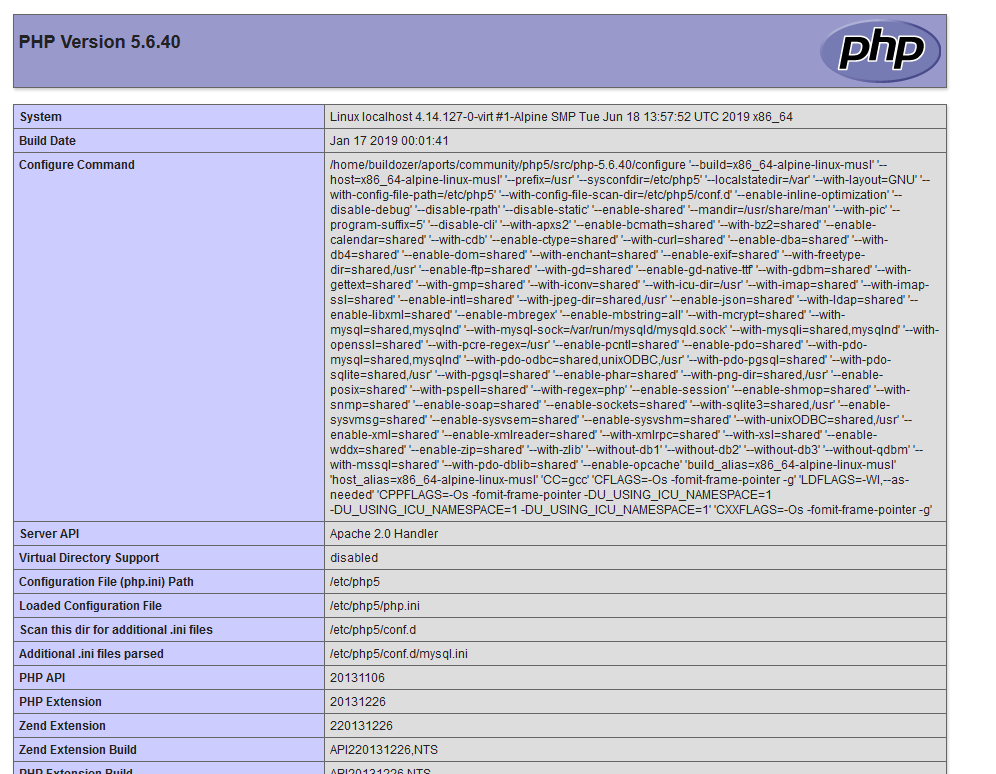
\includegraphics[width=0.5\textwidth]{../images/php2.png}
    \caption{Página info.php renderizada na máquina hospedeira.}
    \label{fig:info.php}
\end{figure}

Uma das configurações que tiveram que ter sido feitas foi a adição de extensões do MySQL e do Ctype no arquivo de configuração do PHP. Para editar o arquivo, utilize o comando na Listagem \ref{lst:php.mysql.ini.caminho} e o conteúdo que foi inserido no arquivo pode ser visualizado na Listagem \ref{lst:php.mysql.ini}. Esta adição foi necessária para que o PHP consiga realizar conexões com o banco e para que ele consiga renderizar corretamente os caracteres em português.

\begin{lstlisting}[language=bash, label=lst:php.mysql.ini.caminho, caption=Abrir no vim o arquivo mysql.ini.]
    vim /etc/php5/conf.d/mysql.ini
\end{lstlisting}

\begin{lstlisting}[label=lst:php.mysql.ini, caption=Conteúdo do arquivo mysql.ini.]
    extension=mysql.so
    extension=mysqli.so
    extension=ctype.so
\end{lstlisting}

\subsubsection{MySQL}\label{mysql}
\begin{wrapfigure}{r}{0.2\textwidth} %this figure will be at the right
    \centering
    
\includegraphics[width=0.2\textwidth]{../images/mysql.png}
\end{wrapfigure}
MySQL é um gerenciador de banco de dados que lida com dados relacionais. 

Infelizmente, a interface do MySQL na imagem do Alpine da versão \textit{20191010} não funcionou. Porém, todas as funcionalidade e extensões necessárias para que o PHP se conecte com um banco funcionaram como esperado.

Para substituir a interface do MySQL, utilizou-se o MariaDB.

\subsubsection{MariaDB}\label{mariadb}
\begin{wrapfigure}{r}{0.2\textwidth} %this figure will be at the right
    \centering
    
\includegraphics[width=0.2\textwidth]{../images/mariadb.png}
\end{wrapfigure}
MariaDB é um gerenciador de banco de dados que lida com dados relacionais. Este foi escolhido como SGDB para lidar com dados do Tematres.

Instalou-se o MariaDB, versão 10.2.24, com o comando listado na Listagem \ref{lst:mariadb.add}.

\begin{lstlisting}[language=bash, label=lst:mariadb.add, caption=Instalação do MariaDB.]
    apk add mariadb
\end{lstlisting}

Para acessar o MariaDB instalado e configurado na versão \textit{20191010} da imagem do Alpine, utiliza-se o comando da Listagem \ref{lst:mariadb.mysql}.

\begin{lstlisting}[language=bash, label=lst:mariadb.mysql, caption=Acessando o MariaDB.]
    mysql -u root -p
    Enter password: root
\end{lstlisting}

% \begin{wrapfigure}{r}{0.5\textwidth}
%     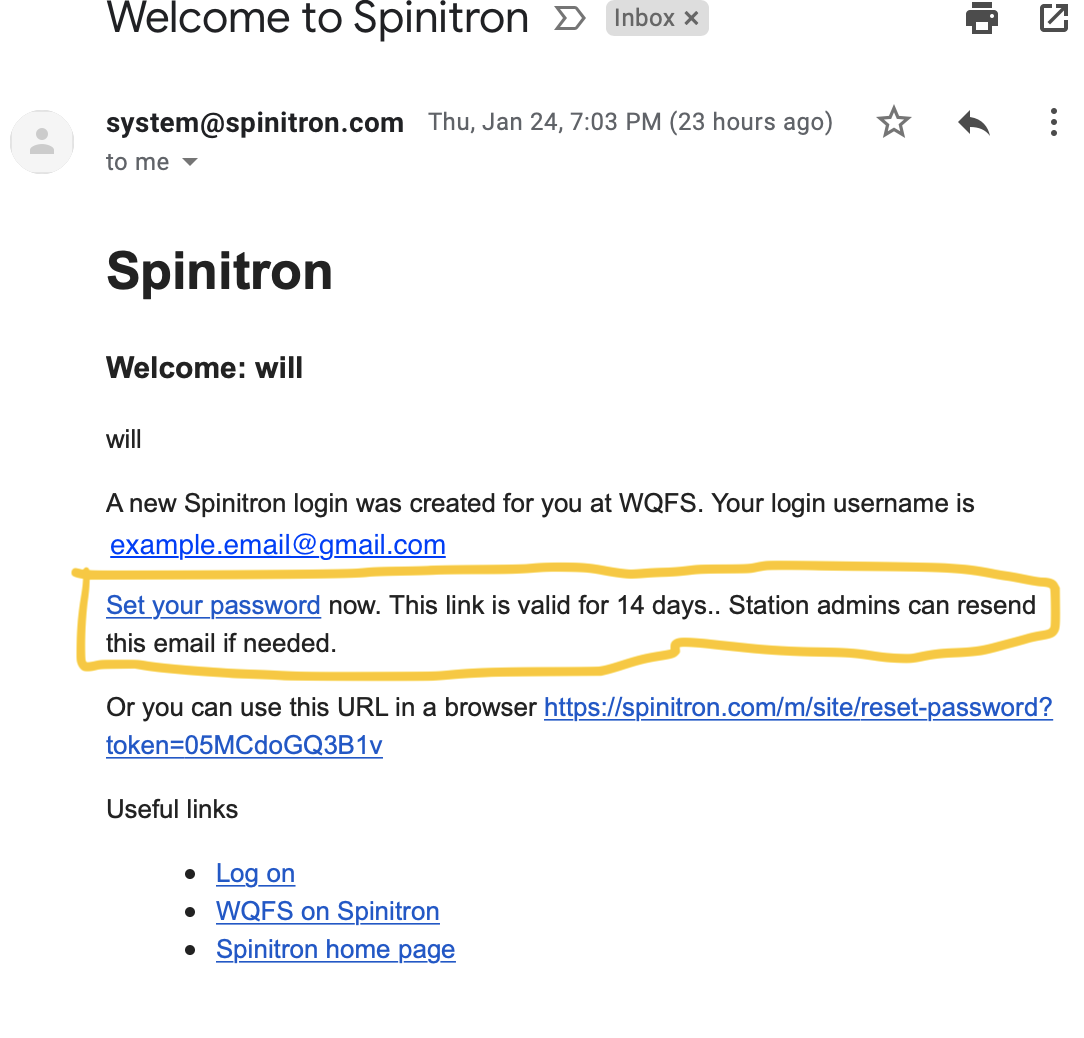
\includegraphics[width=0.5\textwidth]{images/email.png}
%     \caption{Note the link expires after 14 days.}
%     \label{fig2}
% \end{wrapfigure}

% Go to your email and click or copy the link provided by Spinitron. 
% This email should look like Figure~\ref{fig2}

% Remember your email will be your login username.

% Create your password on the page that the link takes you to.

% {\it Please do not forget your password.}

% \clearpage
% \newpage

% \subsection{Logging In}

% %\begin{wrapfigure}{r}{0.45\textwidth}
% %    \includegraphics[width=0.45\textwidth]{images/login_after_password.png}
% %    \caption{The log-in screen.}
% %    \label{fig3}
% %\end{wrapfigure}

%  Next, once you have created your new password Spinitron will take you a page that should look like Figure~\ref{fig3a}. 

% It should say ``New password saved.''

% This is the log-in screen. Enter your email address and password to log in.

% NOTE: sometimes Spinitron will take you to the old version of the website. If that happens, simply click the link that says ``Login for Spinitron v2 is here'' as seen in Figure~\ref{fig3b}

% \begin{figure}[H]
 
%     \begin{subfigure}{0.6\textwidth}
%     \includegraphics[width=0.9\linewidth]{images/login_after_password.png} 
%     \caption{The log-in screen.}
%     \label{fig3a}
%     \end{subfigure}
%     \begin{subfigure}{0.4\textwidth}
%     \includegraphics[width=0.9\linewidth]{images/old_version.png}
%     \caption{The old version of Spinitron.}
%     \label{fig3b}
%     \end{subfigure}
 
% \caption{Login screens.}
% \label{fig:image2}
% \end{figure}

% %\begin{figure}[H]
% %\includegraphics[width=0.40\textwidth]{images/old_version.png}
% %\caption{The old version of Spinitron.}
% %\label{fig4}
% %\end{figure}



% \subsection{Home-Screen and Setup}

% \begin{wrapfigure}{r}{0.45\textwidth}
%     \includegraphics[width=0.45\textwidth]{images/phone_banner.png}
%     \caption{The set phone number banner takes you to the User account page.}
%     \label{fig4}
% \end{wrapfigure}

% Now you are on the Spinitron DJ Home screen. 
% It should look like Figure~\ref{fig4}

% Setup your User account by selecting ``User account'' under the drop-down box under your DJ name or click the ``Please set your phone number.'' banner.

% Make sure you put the correct phone number, this is the number that managers will use to contact you in the future.

% \clearpage
% \newpage

% \subsection{DJ profile}

% (OPTIONAL) Setup your DJ profile. This is accessed using the drop-down box under your DJ name in the top right corner of the page. 
% You can put as much or little information as you like.

% NOTE: Spinitron uses random photos for anything you do not put in a picture for, you are welcome to leave them as they are, delete them, or replace them.

% \begin{figure}[H]
%     \centering
%     \includegraphics[width=0.5\textwidth]{images/Dropdown.png}
%     \caption{The drop-down}
%     \label{fig5}
% \end{figure}

% \begin{figure}[H]
 
%     \begin{subfigure}{0.5\textwidth}
%     \includegraphics[width=1.0\linewidth, height=5cm]{images/DJ_profile1.png} 
%     \label{fig:DJp1}
%     \end{subfigure}
%     \begin{subfigure}{0.5\textwidth}
%     \includegraphics[width=1.0\linewidth, height=5cm]{images/DJ_profile2.png}
%     \label{fig:DJp2}
%     \end{subfigure}
 
% \caption{The DJ profile page}
% \label{fig6}
% \end{figure}